\chapter{Fonctions de 2 (et 3) variables}

\paragraph{} Une fonction de 2 variables réelles est une fonction $f:A \rightarrow \mathbb{R}$ où A est un sous ensemble de $\mathbb{R}^2$.
Son graphes : $\Gamma_f = \{((x, y), f(x, y)) | (x, y) \in A\} \subset \mathbb{R}^3$

\paragraph{Exemple 1} \[\begin{array}{rcl}
f : \mathbb{R}^2 & \rightarrow & \mathbb{R} \\
(x, y) & \mapsto & 2x - y\end{array}\]

graphe : $\{(x, y, z) | (x, y) \in \mathbb{R}^2, z = 2x - y\} = \{(x, y, z) \in \mathbb{R}^3 | 2x -y -z = 0\}$

\begin{wrapfigure}[5]{r}{0pt}
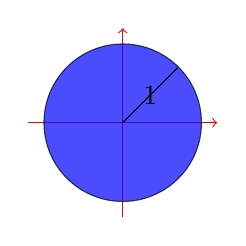
\begin{tikzpicture}
	\draw[->, red] (-1.2, 0) -- (1.2, 0);
	\draw[->, red] (0, -1.2) -- (0, 1.2);
	\draw[fill=blue, opacity=0.7] (0, 0) circle (1);
	\draw[] (0, 0) -- (0.7, 0.7) node [midway] {1};
\end{tikzpicture}
\end{wrapfigure}

\paragraph{Exemple 2} \[\begin{array}{rcl}
f : A & \rightarrow & \mathbb{R} \\
(x, y) & \mapsto & x^2 + y^2 \end{array}\]

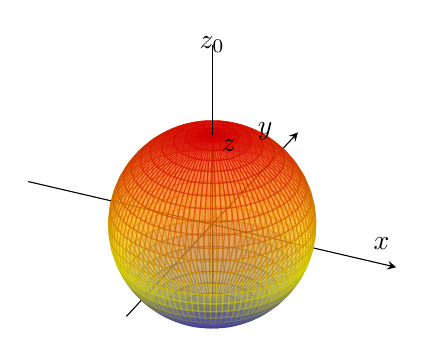
\begin{tikzpicture}
    \begin{axis}[%
        axis equal,
        axis lines = center,
        xlabel = {$x$},
        ylabel = {$y$},
        zlabel = {$z$},
        ticks=none,
    ]
    \addplot3[%
        opacity = 0.5,
        z buffer = sort,
		surf,
        samples = 50,
        variable = \u,
        variable y = \v,
        domain = 0:180,
        y domain = 0:360,
    ]
    ({cos(u)*sin(v)}, {sin(u)*sin(v)}, {cos(v)});
	\draw[] (current plot begin) --+ (axis direction cs:0,0,1) node {$z_0$};
    \end{axis}
\end{tikzpicture}
graphe de $f$

\paragraph{Notation} $r > 0, (x_0, y_0) \in \mathbb{R}^2$

\[D \subset \mathbb{R}^2 = \{(x, y) \in \mathbb{R}^2 | (x-x_0)^2 + (y-y_0)^2 < r^2\]

Avec D le disque centré en $(x_0, y_0)$ de rayon $r$, sans son bord.

\paragraph{Définition} On dit que $(x_0, y_0)$ est \ul{adherent} à $A \subset \mathbb{R}^2$ \ul{si} : \[\forall \delta > 0, D((x_0, y_0), \delta) \cap A \neq 0\]

\paragraph{Exemple} (cf A de l'exemple 2)

L'ensemble des points adhérents à A est $\{(x, y) \in \mathbb{R}^2 | x^2 + y^2 \leq 1\}$

("$A \cup$ est son bord")

\paragraph{Définition} On dit que f \ul{tend vers l} $\in \mathbb{R}$ quand (x, y) tend vers $(x_0, y_0)$ si et seulement si $\forall \epsilon > 0, \exists \delta > 0$ tel que \[\forall (x, y) \in D((x_0, y_0), \delta), |f(x, y) - l| < \epsilon\]

Et on note alors $\lim_{(x, y) \to (x_0, y_0)} f(x, y) = l$

\paragraph{Définition} $f:A \rightarrow \mathbb{R} (A \subset \mathbb{R}^2)$ est \ul{continue} en $(x_0, y_0) \in A$ si $\lim_{(x, y) \to (x_0, y_0)} f(x, y) = f(x_0, y_0)$.

\paragraph{Propriété} $f, g : A \rightarrow \mathbb{R}, (x_0, y_0) \in A$

\begin{itemize}
	\item $f+g$, $f\cdot g$ sont continues en $(x_0, y_0)$
	\item Si $g(x_0, y_0) \neq 0$, $\frac{f}{g}$ est continue en $(x_0, y_0)$
\end{itemize}

\paragraph{Définition} $f:A \rightarrow \mathbb{R}, A \subset \mathbb{R}^2, (x_0, y_0) \in A$

f est \ul{differentiable} en $(x_0, y_0)$ s'il existe \begin{itemize}
	\item $(a, b)  \in \mathbb{R}^2$
	\item $\epsilon D((x_0, y_0), \delta) \rightarrow \mathbb{R}$ avec $\epsilon(x, y) \xrightarrow[]{(x, y) \to (x_0, y_0)} 0$
\end{itemize}

tel que : \[f(x, y) = f(x_0, y_0) + a(x-x_0) + b(y-y_0) + ||(x-x_0, y-y_0)|| \epsilon(x, y)\]

\paragraph{Remarque} Si $f : \mathbb{R} \rightarrow \mathbb{R}, x_0 \in \mathbb{R}$. 

f est dérivable en $x_0$ si $\lim_{x \to x_0} \frac{f(x) - f(x_0)}{x-x_0}$ existe, c'est à dire \[\exists a \in \mathbb{R} \text{ tel que } f(x) = f(x_0) + a(x-x_0) + (x-x_0) \epsilon(x)\]

\paragraph{Définition}
Si A ne contient que des points "intérieurs", f est différentiable sur A si elle est différentiable en tout $(x_0, y_0) \in A$

Si $f$ est différentiable en $(x_0, y_0), (h, k) \mapsto ah + bk$ est la différentielle de f.

\paragraph{Remarque 2} différentiabilité peut aussi s'exprimer sous la forme : \[f(x_0+h, y_0+k) = f(x_0, y_0) + ah+bk + ||(h, k)|| \epsilon(h, k)\]

avec $\epsilon : D((0, 0), \delta) \to \mathbb{R}$ et $\epsilon(h, k) \xrightarrow[]{(h, k) \to (0, 0)} 0$

$h = x-x_0, k=y-y-0$

Si f est différentiable en $(x_0, y_0)$, On note sa différentielle par $df(x_0, y_0)$ ou $d_{(x_0, y_0)}f$.

\paragraph{Remarque} $f(x, y) = f(x_0, y_0) + d_{(x_0, y_0)}f(h, k) + ||(h, k)||\epsilon(h, k)$

\paragraph{Remarque} \[\begin{array}{rcl}
	d_{(x_0, y_0)}f(h, k) &=& ah + bk \\
	&=& \begin{pmatrix}
a \\
b\end{pmatrix} \cdot \begin{pmatrix}
h \\
k\end{pmatrix}\end{array}\]

$\begin{pmatrix}
a\\
b\end{pmatrix}$ est le gradiant de f en $(x_0, y_0)$, noté $\vec{grad}(f) (x_0, y_0)$ ou $\vec{\bigtriangledown}_{(x_0, y_0)} f$

\paragraph{Récapitulatif} $d_{z_0} f(h, k) = \vec{\bigtriangledown}_{z_0}f \cdot\begin{pmatrix}
h \\
k\end{pmatrix}$ avec $z_0 = (x_0, y_0)$

\[f'(z_0)(h) = f'(z_0)\cdot h\]

\paragraph{Exemple}

\[\begin{array}{rcl}
	f:\mathbb{R}^2 &\rightarrow &\mathbb{R}\\
	(x, y) &\mapsto& x^2 + y^2\end{array}\]

$\vec{\bigtriangledown}_{(x_0, y_0)} f = \begin{pmatrix}
2x_0 \\
2y_0\end{pmatrix}$

\[\underbrace{f(x_0+h, y_0+k)}_{(x_0+h)^2 + (y_0+h)^2} = f(x_0, y_0) + d_{(x, y_0)}f(h, k) + || (h, k)||\epsilon(h, k)\]

\[\begin{array}{rcl}
	x_0^2 + 2x_0h + h^2 + y_0^2 + 2y_0^k + k^2 &=& \underbrace{(x_0^2 + y_0^2)}_{ f(x_0, y_0)}  + \underbrace{(2x_0^h + 2y_0k)}_{d_{(x_0, y_0)}f(h, k)}  + \underbrace{h^2 + k^2}_{?} \\
h^2 + k^2 &=& ||(h, k)||\epsilon(h, k) \\
				&=& \sqrt{h^2 + k^2}\end{array}\]

On pose $\epsilon(h, k) = \sqrt{h^2 + k^2}$

